% CVS: $Id: lrec08.tex,v 1.8 2008/03/26 07:26:49 rpnlpir Exp $
%
% CVS: $Log: lrec08.tex,v $
% CVS: Revision 1.8  2008/03/26 07:26:49  rpnlpir
% CVS: with Isaac's edits.  Waiting for small edits.
% CVS:
% CVS: Revision 1.7  2008/03/20 02:08:51  rpnlpir
% CVS: Partial commit.
% CVS:
% CVS: Revision 1.6  2008/03/18 15:48:05  rpnlpir
% CVS: Added partial evaluation section. -M
% CVS:
% CVS: Revision 1.5  2008/02/25 06:52:54  rpnlpir
% CVS: *** empty log message ***
% CVS:
% CVS: Revision 1.4  2007/10/31 05:00:50  rpnlpir
% CVS: All done, submitted.
% CVS:
% CVS: Revision 1.3  2007/10/31 01:36:31  rpnlpir
% CVS: spell checked. going to submit.
% CVS:
% CVS: Revision 1.2  2007/10/31 01:28:38  rpnlpir
% CVS: Isaac and Lee's edits.
% CVS:
%
\documentclass[10pt, a4paper]{article}
\usepackage{lrec2006}
\usepackage{epsfig}
% \pagenumbering{arabic}						%BUG: Take out before submitting!!!

% BUG: for finished papers, a) spell check, b) check hypenation of noun mods, c) e.g., 

\begin{document}

\title{ParsCit: An open-source CRF reference string parsing package}

\name{Isaac G. Councill$^{\ast}$, C. Lee Giles$^{\ast}$, Min-Yen Kan$^{\dagger}$}

\address{$^{\ast}$ College of Information Sciences \& Technology \\
         The Pennsylvania State University \\
         \{icouncil,giles\}@ist.psu.edu \\ \\
         $^{\dagger}$Department of Computer Science \\
         National University of Singapore \\  
         kanmy@comp.nus.edu.sg}

\abstract{We describe ParsCit, a freely available, open-source
implementation of a reference string parsing package.  At the core of
ParsCit is a trained conditional random field (CRF) model used to
label the token sequences in the reference string.  A heuristic model
wraps this core with added functionality to identify reference strings
from a plain text file, and to retrieve the citation contexts.  The
package comes with utilities to run it as a web service or as a
standalone utility.  We compare ParsCit on three distinct reference
string datasets and show that it compares well with other previously
published work.}

%%%%%%%%%%%%%%%%%%%%%%%%%%%%%%%%%%%%%%%%%%%%%%%%%%%%%%%%%%%%%%%%%%%%%%

\maketitleabstract

\section{Introduction}

In scholarly works, we acknowledge the past contribution of fellow
scientists by referring to their work through formal citations.  Scientific papers often
conclude with a section that lists referenced works in the form of a
reference list or bibliography.  This form of acknowledgment is
crucial in helping readers and reviewers to relate the current work to
its context within the research community's discourse.

An ongoing focus within the bibliographic research community is the
automatic creation of citation networks from underlying source documents. A
prerequisite to programatically recovering links between referring and
referred-to documents requires a machine to understand the structure
of the strings in a reference section.  Each reference
string\footnote{We use ``reference string'' to refer to an item in the
reference section at the end of a document, and``citation'' to refer
to the pointers used in the body of the main text of a document.} can
be viewed as a set of fields (e.g., author, title, year, journal) that
are represented as a surface string, with implicit cues such as
punctuation to assist in recovering the encoded data.  While parsing
these reference strings at the end of a document is often
straightforward for human readers, the sheer diversity of different
standards espoused by different communities, coupled with inadvertent
errors on the part of authors, makes this process difficult to automate.

Many methods have been proposed to deal with this sequence labeling
problem \cite{peng04accurate,276685}.  In this paper we describe our
implementation of ParsCit, a system that uses a core of machine
learned methods coupled with a heuristic processing framework.  While
many methods that use machine learning have been proposed for this
exact problem \cite{huang04:_extrac_citat_metad_onlin_public,1255219},
our contribution lies in 1) devising new features useful for this
problem, 2) automatically extracting citation contexts, 3) packaging
our results as a software module that can be called on a standalone
basis or as a web service, and 4) making our code open-source for the
community's benefit.

In the remainder of this paper, we discuss the core learning model,
and detail the pre- and post-processing steps that wrap the sequence
labeling model into a working service.  We then describe the
implementation details and usage of the toolkit, and conclude with a
comparison with related work.

\section{Learning Model}

We first formally define the problem to be solved. We say that a
reference string $R$ is first broken down into a sequence of tokens
$\{r_1, r_2, ..., r_n\}$.  Each token is to be assigned the correct
label from a set of classes $C$ = $\{c_1, c_2, ..., c_m\}$.  Evidence used
in classifying some token $r_i$ can be any data that can be derived
from the surface reference string, as well as previously-assigned $r_1
... r_{i-1}$ classifications.

This sequence labeling problem is common to a large set of NLP tasks,
including part-of-speech tagging, chunking, and semantic role
labeling.  It also embodies the reference parsing problem tackled
here, in which the classes are the metadata fields such as author,
title, journal, etc.  In our implementation, a total of 13 classes are
labeled, corresponding to common fields used in bibliographic reference
management software (e.g., EndNote, BibTeX).

We use a conditional random field~\cite{655813} formalism to learn a model
from labeled training data that can be applied to unseen data.  This
learning model scales well, handling large sets of possibly
overlapping (i.e., conditionally dependent) features.  We have
engineered our features to rectify the classification errors made by
models created from previous work.  We list the general category of
features used by the ParsCit system below; the number of individual
features used to represent each category are given in parentheses.

\begin{description}
\item [Token identity (3):] We encode separate features for each
token in three different forms: 1) as-is, 2) lowercased, and 3)
lowercased stripped of punctuation.
\item [N-gram prefix/suffix (9):] We encode 4 features for the first 1-4
characters of the token, similarly for the last 1-4 characters.  A
single feature also examines the last character of the token, encoding
whether it is uppercase, lowercase or numeric.
\item [Orthographic case (1):] We analyze the case of the token,
assigning it one of four values: $Initialcaps$, $MixedCaps$,
$ALLCAPS$, or $others$.
\item[Punctuation (1):] Similarly, we give fine-grained distinctions
for the punctuation present in token: $leadingQuotes$, $endingQuotes$,
$multipleHyphens$ (occasionally found in page ranges),
$continuingPunctuation$ (e.g., commas, semicolons), $stopPunctuation$
(e.g., periods, double quotes), $pairedBraces$, $possibleVolume$ (e.g.,
``3(4)''), or $others$.
\item [Number (1):] We analyze the token for possible numeric
properties.  The value of this feature can be specific, such as $year$
(a value between 19xx and 20xx), $possiblePageRange$ (contains
$[0-9]-[0-9]$), $possibleVolume$ (contains $[0-9]([0-9]*)$), $ordinal$
(contains number followed with a suffix such as ``th''), or a general
class: $4digit$, $3digit$, $2digit$, $1digit$, $hasDigit$ or
$noDigits$.  
\item[Dictionary (6):] Separate analyzers check whether the token
is a key within a hash table of possible publisher names, place names,
surnames, female and male names, and months. 
\item[Location (1):] We code the relative location of the token within
the reference string, discretized into $n$ uniform bins ($n$ was set
to 12 by experimentation).  In most styles, more important data such
as author, title, year is placed towards the beginning of the citation
string; this feature attempts to capture regularities in position on
top of the sequence labeling strengths of the CRF learner.
\item[Possible editor (1):] This feature indicates whether a token
such as ``eds.'' is present anywhere within the reference string.  
\end{description}

Note that many of our features make fine-grained distinctions (e.g.,
orthographic case, numeric, punctuation evidence); these increase
performance significantly over previous work.  We also observe that
misclassifications of editors for authors occur often in previous
work; to correct for this, we explicitly model the possible editor
feature so that long-range dependencies are factored out.

Features are applied to the current token to be tagged and, for
important features, applied to a contextual window of words (window
width of -2 to +2).  We use the freely-available CRF++
package\footnote{http://crfpp.sourceforge.net/}, which makes the
application of the feature inventory across multiple tokens easy.
This implementation of the CRF learning model was also selected as it
is licensed using the Lesser GNU Public License (LGPL), which is
suitable to be embedded in free and commercial products.

\section{Pre-Processing Steps}

Before reference strings can be properly extracted, it is necessary to
first find the references within an article. Although formatting
(e.g., font changes) may be of significant help, dependency on
specific formatting may lead to a loss of generality.  For this
reason, ParsCit assumes only that documents are first converted to
plain text, encoded using UTF-8.  Well-formed text extraction is
notoriously difficult to do with certain types of files (e.g., PDF
files), but it is a critical requirement for proper extraction.

Given a plain UTF-8 text file, ParsCit finds the reference strings
using a set of heuristics.  It begins by searching for a labeled
reference section in the text. Labels may include such strings as
``References'', ``Bibliography'', ``References and Notes'', or common
variations of those strings. Text is iteratively split around strings
that appear to be reference section labels. If a label is found too
early in the document according to a configurable parameter (under
40\% of the whole text, by default) , subsequent matches are sought.
The final match is considered the starting point of the reference
section.  Processing then begins to find the end point by searching
for subsequent section labels, such as appendices, figures, tables,
acknowledgments, autobiographies, etc., or the end of the document.

Once the complete reference section is extracted, the next phase is to
segment individual reference strings. There are three general cases
for reference string segmentation: 1) strings are marked with square
bracket or parenthetical reference indicators (e.g., ``[1]'', ``(1)'',
``[Heckerman02]'', etc.), 2) strings are marked with naked numbers
(e.g. ``1'' or ``1.''), and 3) strings are unmarked (such as in APA
style). The first step is therefore to find the marker type for the
citation list. This is done by constructing a number of regular
expressions matching common marker styles for cases 1 and 2, then
counting the number of matches to each expression in the reference
string text. If either case yields more matches than 1/6 of the total
lines in the citation text, the case with the greatest number of
matches is indicated. In both cases, the same regular expressions that
were used to find the marker type may be used to indicate the starting
point of a citation, and citations are segmented in this manner. If no
reference string markers are found, several heuristics are used to
decide where individual strings start and end based on the length of
previous lines (short length indicates a possible final line of a
reference string), strings that appear to be author name lists
(usually found at the beginning of unmarked citations), and ending
punctuation (the final line of citation usually will end with a
period.

The list of individual reference strings is then written out and the
CRF++ model as discussed earlier is applied to the data.

\section{Post-Processing Steps}

Based on the output of running CRF++, several steps are necessary to
normalize each tagged field into a standard representation. Author
names may occur in various orders and formats in reference strings,
such as ``M.-Y. Kan and I. G. Councill'' or ``Kan, M.-Y. \& Councill,
I. G.''. The name string must first be segmented into individual names
based on an analysis of separator locations (e.g., comma or semicolon
placement). Each name is then normalized to the form ``M-Y Kan'' and
``I G Councill''. Number fields such as publication volume and number
are normalized such that only the numeric value is preserved
(e.g. ``vol. 5'' is normalized to ``5''). Similarly, only the year
portion of date fields is preserved. Finally, page numbers are
normalized into the form ``start--end'', such that a field
``pp. 584-589'' becomes ``584--589''.

\section{Extracting Citation Contexts}

Based on the reference marker that was discovered during reference
segmentation or generated during post-processing, one or more regular
expressions are generated that can be used to scan the body text for
citations to a particular reference string. These expressions vary based
on the three types of markers (corresponding to the three cases for
reference string segmentation above). For markers explicitly tagged with
square bracket or parenthetical markers in the reference section, the
markers are converted into regular expressions directly. Naked number
markers (e.g., ``1'' or ``1.'') are converted into square bracket and
parenthetical expressions. In the case of naked numbers, priority is
given to the square bracket representation, and the parenthetical
expression will not be applied if square bracket matches occur in the
body text. The marker expressions are flexible enough to handle cases
where a match occurs in a list of references (e.g., ``[12, 2, 5]'')
without matching the same numbers outside of the reference context
(e.g., ``see Figure (2)'').

Finally, markers from unmarked citation lists (such as in APA style)
will be generated based on the last names of the authors and year of
publication. Various forms of the marker will be created, such that a
paper authored by Poljak, Rendl, and Wolkowicz in 1994 will yield the
following markers: 1) ``Poljak, Rendl, Wolkowicz, 1994'', 2) ``Poljak,
Rendl, and Wolkowicz, 1994'', 3) ``Poljak, Rendl, \& Wolkowicz, 1994'',
and 4) ``Poljak et al., 1994''. Some added flexibility regarding
omitted punctuation is built into the regular expressions but is not
included here for clarity.

Each regular expression is then applied to the body text to generate a
list of all context matches. The size of the context string is
configurable, but by default extends to 200 characters on either side
of the match. For the sake of efficiency when faced with long
documents, matching will cease after a configurable number of matches
are found.

\section{Usage and API}

ParsCit includes command line utilities for extracting reference
strings from text documents. By default, text files are expected to be
encoded in UTF-8, but the expected encoding can be adjusted using perl
command line switches. To run ParsCit on a single document, users simply
execute a single command:

\vspace{.2cm}
\parbox[h]{\columnwidth}{{\tt citeExtract.pl textfile [outfile]}}
\vspace{.2cm}

If ``outfile'' is specified, the XML output will be written to that
file; otherwise, the XML will be printed to standard output.

There is also a web service interface available, using the SOAP::Lite
perl module. To start the service, one executes:

\vspace{.2cm}
\parbox[h]{\columnwidth}{{\tt parscit-service.pl}}
\vspace{.2cm}

A Web Service Definition Language (WSDL) file is provided with the
distribution that outlines the message details expected by the ParsCit
service for use by developers. Expected parameters in the input
message are ``filePath'' (a path to the text file to parse) and
``repositoryID''. The ParsCit service is designed for deployment in an
environment where text files may be located on file systems mounted
from arbitrary machines on the network. Thus, ``repositoryID''
provides a means to map a given shared file system to its mount
point. Repository mappings are configurable. The ``filePath''
parameter provides a path to the text file relative to the repository
mount point. The local file system may be specified using the reserved
repository ID ``LOCAL''. In that case, an absolute path to the text
file may be specified.

Both perl and ruby clients are also provided that demonstrate how to
use the service. For example, one can execute the perl client with the
following command:

\vspace{.2cm}
\parbox[h]{\columnwidth}{{\tt parscit-client.pl filePath repositoryID}}
\vspace{.2cm}

If the call is successful, the XML output will be printed to standard
output.

The ParsCit libraries may be used directly from external
perl applications through a single interface module.  If XML
output is desired (the default), the ParsCit::Controller::extractCitations
(\$filePath) subroutine will suffice. If it is desirable to have faster, more
structured access to citation data from the external code, a
more convenient implementation, ParsCit::Controller::extractCitationsImpl
(\$filePath), is provided. Rather than returning the data in XML
representation, the parameters returned are a status code (code > 0
indicates success), an error message (blank if no error), a reference
to a list of ParsCit::Citation objects containing the parsed citation
data, and a reference to the body text identified during
pre-processing for subsequent context analysis or indexing.

\section{Evaluation}

An evaluation of ParsCit performance can take place at two levels:
the raw sequence decoding performance of the underlying CRF model
or the normalized output after application-level post-processing.
Most previous work centers
on the core task of reference string parsing, but does not
include evaluations of field normalizations such as author delimitation or retrieval of citations
contexts.  These two latter features are core aspects of ParsCit that
make it eminently suited for direct incorporation in external digital
library software and frameworks.  However, in order to make direct
comparisons with other work we limit our discussion to
published results on reference parsing using publicly available
datasets.  This limits us to evaluating ParsCit on three different
datasets of reference strings available for the computer science domain
and analyzing performance on the CRF sequence decoding alone.

\subsection{Cora}

The Cora dataset is derived from one of the first studies in automated
reference string parsing
\cite{seymore99:_learn_hidden_markov_model_struc_infor_extrac}.  This
dataset created a gold standard for 200 reference strings sampled from
various computer science publications.  These citations were segmented
into thirteen different fields -- ``author'', ``booktitle'', ``date'',
``editor'', ``institution'', ``journal'', ``location'', ``note'',
``pages'', ``publisher'', ``tech'', ``title'', and ``volume'' --
reflective of BibTeX fields that might be used to generate the
references themselves.  Table \ref{t:eval-cora} gives the field
accuracy and F$_1$ of ParsCit, trained using ten-fold cross
validation, compared to the original CRF-based system
\cite{peng04accurate} that inspired our work.  Note that the Cora
dataset does not further segment the author field into individual
authors; so our evaluation is done by regarding any contiguous
``author'' fields as a single field.

\begin{table}[htb]
\centering
\begin{tabular}{|l|c|c|c|c|c|}
\hline
Field & \multicolumn{3}{|c|}{ParsCit} & \multicolumn{2}{|c|}{Peng} \\
& Precision & Recall & $F_1$ & Acc. & $F_1$ \\ 
\hline
Author 		& 98.7 & 99.3 & .99 	& 99.9 & .99 \\
Booktitle 	& 92.7 & 94.2 & .93	& 97.7 & .94 \\
Date 		& 100 & 98.4 & .99	& 99.8 & .99 \\
Editor 		& 92.0 & 81.0 & .86	& 99.5 & .88 \\
Institution 	& 90.9 & 87.9 & .89 	& 99.7 & .94 \\
Journal 	& 90.8 & 91.2 & .91 	& 99.1 & .91 \\
Location 	& 95.6 & 90.0 & .93	& 99.3 & .87 \\
Note 		& 74.2 & 59.0 & .65	& 99.7 & .81 \\
Pages 		& 97.7 & 98.4 & .98 	& 99.9 & .99 \\
Publisher 	& 95.2 & 88.7 & .92 	& 99.4 & .76 \\
Tech 		& 94.0 & 79.6 & .86 	& 99.4 & .87 \\
Title 		& 96.0 & 98.4 & .97 	& 98.9 & .98 \\
Volume 		& 97.3 & 95.5 & .96 	& 99.9 & .98 \\
\hline
Average* 	& 95.7 & 95.7 & .95	& -- & .91\\
\hline
\end{tabular}
\caption{Field reference string parsing performance on the Cora dataset using 10-fold cross validation.  Averages are micro averages for ParsCit and macro averages for \cite{peng04accurate}.}
\label{t:eval-cora}
\end{table}

We follow the the experimental methodology of the original experiments
done in \cite{peng04accurate} as closely as possible, using ten-fold
cross validation with 50-line slices of the training data. The results
above show that the core module of ParsCit that performs reference
string segmentation performs satisfactorily, and is largely comparable to
Peng and McCallum's original CRF based system.  The publicly-available
implementation of ParsCit comes loaded with a model trained over the
full Cora dataset.

\subsection{CiteSeer$^X$}

In order to characterize ParsCit's performance within its largest deployment
context, CiteSeerX, a separate data set was generated by randomly sampling
200 reference strings from the approximately 14 million strings within the
CiteSeerX system at the time of the evaluation.  Each reference string was
manually labeled in the very same manner as the Cora data set.  This sample
contains reference strings in a wide variety of formats.  Table \ref{t:eval-csx}
shows the results of applying ParsCit to the CiteSeerX data set.  
Interestingly, performance
deteriorates significantly for all fields, indicating that the Cora data set may not
be representative of the variety of reference string formats found within the
computer science domain.  However, results are still good for most fields and very
good for author, title, and date fields, which are the most critical fields for
citation matching, a hallmark feature of the CiteSeerX and Cora systems.

Further analysis of the mistakes that were made on the CiteSeerX data set
reveals that most errors affect only small portions of the reference string decoding.
Approximately 51\% of the strings were decoded perfectly.  For the 49\% of
strings where mistakes were made, Figure \ref{f:errorPercents} shows the
distribution of the percentage of tokens within the strings that were misclassifed,
showing that only a small percentage of strings were damaged by more than
25\%.  Figure \ref{f:fieldErrors} further shows that only 7\% of all strings contained
misclassifications in more than two separate fields.

\begin{table}[htb]
\centering
\begin{tabular}{|l|c|c|c|}
\hline
Field & Precision & Recall & F$_1$ \\
\hline
Author	& 95.8	& 95.7	& .96 \\
Booktitle	& 72.5	& 92.9	& .81 \\
Date	& 98.8	& 89.8	& .94 \\
Editor	& 95.6	& 51.1	& .67 \\
Institution	& 70.9	& 76.7	& .74 \\
Journal	& 88.0	& 78.6	& .83 \\
Location	& 91.9	& 78.4	& .85 \\
Note	& 88.9	& 17.2	& .29 \\
Pages	& 90.3	& 91.5	& .91 \\
Publisher	& 88.7	& 74.8	& .81 \\
Tech	& 76.1	& 70.0	& .73 \\
Title	& 91.9	& 93.9	& .93 \\
Volume	& 89.3	& 85.0	& .87 \\
\hline
\end{tabular}
\caption{Field reference string parsing performance on the CiteSeer$^X$ dataset.}
\label{t:eval-csx}
\end{table}

\begin{figure}[htb]
\centering
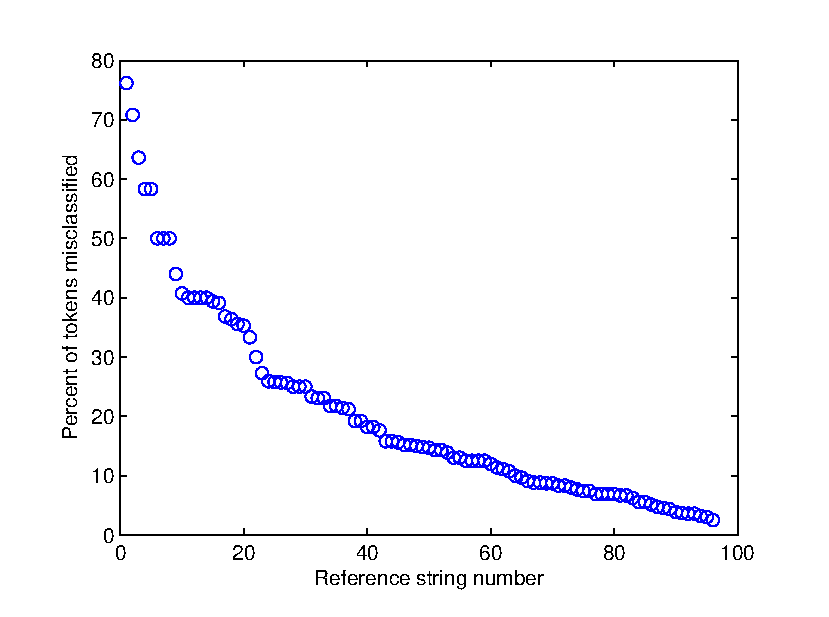
\epsfig{file=errorPercents.eps,width=\columnwidth}
\caption{On those citation strings where mistakes are made
(roughly half), this shows the distribution of the percentage of
tokens misclassified by ParsCit.}
\label{f:errorPercents} 
\end{figure}

\begin{figure}[htb]
\centering
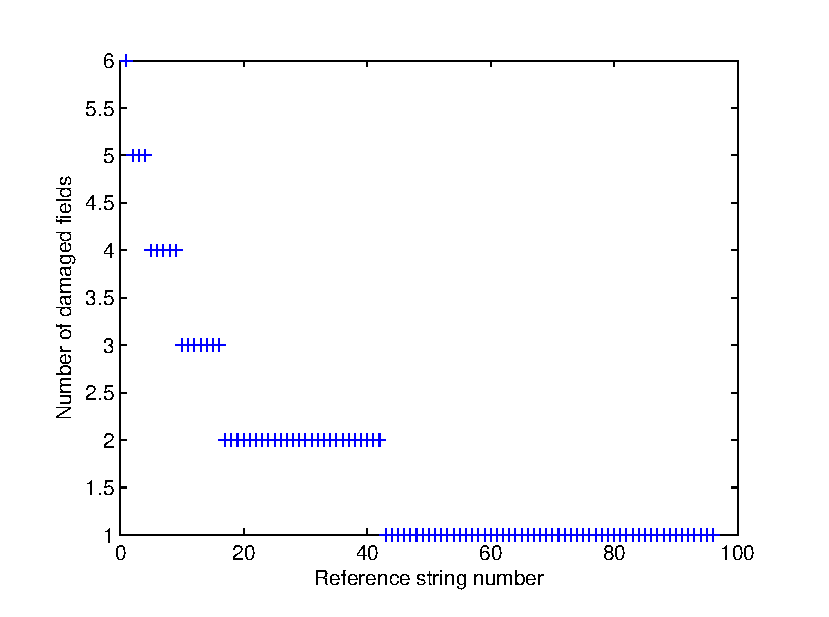
\epsfig{file=fieldErrors.eps,width=\columnwidth}
\caption{On those citation strings where mistakes are made, this
shows the distribution of the number of fields that were damaged by
misclassifications.  Only about 7\% of citations in the test set are
damaged in more than 2 fields.}
\label{f:fieldErrors}
\end{figure}

\subsection{FLUX-CiM} 

The FLUX-CiM authors \cite{1255219} use two different datasets to
evaluate their unsupervised reference string parsing system: a health
sciences dataset and a computer science dataset.  Unlike FLUX-CiM,
ParsCit is a supervised system and can be re-trained for the
particularities of the Health Science domain.  As we have yet to
complete the preparation work necessary for re-training, we have only
compiled the FLUX-CiM results for CS dataset, as the domain matches
the Cora dataset.  FLUX-CiM reports accuracies and F$_1$ scores
for each type of field, but additionally segments contiguous authors
as individual fields.  FLUX-CiM annotates ten fields, differing
from Cora's thirteen.  A crosswalk to convert Cora annotation to
FLUX-CiM was generated (collapsing ``editors'' with ``authors'';
``institution'' with ``publisher''; omitting ``note'' and ``tech'';
and expanding ``volume'' to differentiate between ``volume'' and
``number'').

The FLUX-CiM CS dataset was ``gathered [from] a heterogenous
collection composed by assorted references from several conferences
and journals in [computer science] area.''  The dataset has 300
instances, of which 14 are duplicates.  Since no gold-standard markup
was available, we retagged the provided raw input strings using the
crosswalk.  We then applied ParsCit (trained on the Cora model) to
test its performance against FLUX-CiM.  We follow their evaluation
metrics and report field-specific precision, recall and F$_1$ values.

\begin{table*}[htb]
\centering
\begin{tabular}{|l|c|c|c|c|c|c|c|}

\hline
Field & \multicolumn{3}{|c|}{ParsCit} & \multicolumn{3}{|c|}{FLUX-CiM} \\
& Precision & Recall & $F_1$ & Precision & Recall & $F_1$ \\ 

\hline
Author	& 98.8 & 99.0 & .99	& 93.5 & 95.6 & 0.95 \\
Title 	& 98.8 & 98.3 & .96	& 93.0 & 93.0 & 0.93 \\
Journal	& 97.1 & 82.9 & .89	& 95.7 & 97.8 & 0.97 \\
Date 	& 99.8 & 94.5 & .97 	& 97.8 & 97.4 & 0.98 \\
Pages 	& 94.7 & 99.3 & .97 	& 97.0 & 97.8 & 0.97 \\
Conference(Booktitle)	& 95.7 & 99.3 & .97 	& 97.4 & 95.4 & 0.96 \\
Place(Location)	& 96.9 & 88.4 & .89	& 96.8 & 97.6 & 0.97 \\
Publisher 	& 98.8 & 75.9 & .85 	& 100.0 & 100.0 & 1.00 \\
Number 	& -- & -- & --	&  97.9 & 97.9 & 0.98 \\
Volume 	& 95.3 & 89.7 & .92	&  100.0 & 98.2 & 0.99 \\
\hline
Average & 97.4 & 97.4 & .94 	& 96.9 & 97.1 & 0.97 \\
\hline
\end{tabular}
\caption{Field reference string parsing performance on the FLUX-CiM dataset.}
\label{t:fc-eval}
\end{table*}

Statistics for FLUX-CiM are replicated from their published work;
ParsCit's field accuracy is compiled using the {\tt conlleval.pl}
script provided by the CoNLL conference shared tasks on chunk
labeling.  Table \ref{t:fc-eval} shows that ParsCit compares favorably
against FLUX-CiM on the key common fields of ``author'' and ``title'', as was
seen in the CiteSeer$^X$ dataset.  Key errors that the system makes in
comparison with FLUX-CiM is in not segmenting ``volume'', ``number'' and
``pages'', as ParsCit currently does not further tokenize beyond
whitespaces in the reference string (e.g., ``11(4):11-22'' versus ``11
(4) 11 - 22'').  FLUX-CiM does and is able to distinguish these fields
more accurately.  We plan on incorporating some preprocessing
heuristics to ParsCit to correct for such errors.

\section {Related Work}

The problem of citation parsing has been the focus of several research
initiatives
\cite{97:_univer_citat_datab_catal_refor_schol_commun,lawrence99:_digit_librar_auton_citat_index}.
We examine existing citation parsers, which can be generally divided
into two categories: template matching and machine learning based
approaches.
 
A {\it template matching approach} takes an input citation and matches
its syntactic pattern against known templates. The template with the
best fit to the input is then used to label the citation's tokens as
fields.  The canonical example of a template based approach is
ParaTools~\cite{jewell00:_parac}, a set of Perl modules to perform
reference string parsing.  ParaTools contains 400 templates to match
reference strings to, but even this large amount manifests coverage
problems.  While users may choose to add new templates to ParaTools
manually, the process is cumbersome and unscalable.  The fact that
authors may not strictly adhere to citation styles or that text
extraction or OCR may produce reference strings that do not adhere to
the templates also diminishes this utility.  A further weakness of
ParaTools is that it tags ambiguous fields as ``Any'', equivalent to
not tagging the token at all.
\cite{huang04:_extrac_citat_metad_onlin_public} report ParaTool's
precision as approximately 30\%.  This level of performance and lack
of portability make the approach unsuitable for high volume data
processing.

The limitations of the template-based approach have encouraged
researchers to try {\it supervised machine learned models} for
citation parsing.  Given sufficient training data, a machine-learned
parser can produce high performance in accuracy, regardless of
citation styles.  We review four systems published in recent years
that deal with this work.

Seymore {\it et al.}
\shortcite{seymore99:_learn_hidden_markov_model_struc_infor_extrac}'s work
led to the creation of the Cora dataset.  Their approach used a Hidden
Markov Model (HMM) to build a reference string sequence labeler.
Unlike a standard HMM, they propose and validate performance
improvements when using internal states for different parts of the
field (similar to IOB encoding on other labeling tasks).  In later
work by the same group, Peng and McCallum \shortcite{peng04accurate} used
the reference string parsing task as a benchmark for testing
Conditional Random Fields (CRF).  Their work established CRFs as
strong learning model for this task.  This work motivates our choice
of a CRF as the base learning model for ParsCit.

The first version of ParsCit used Maximum Entropy (ME) training to
compute a model \cite{ng04:_citat_parsin_using_maxim_entrop_repair}.
Aside from using ME, which can be seen as a step towards a
discriminative version of Hidden Markov Models, this work featured two
rounds of prediction: a first round to label a reference string itself
and a second, global round, that takes into account how other
reference strings nearby (e.g., in a Reference or Bibliography
section) were labeled by the first round.  This approach is the only
one that tries to take advantage of such information, which may prove
useful in cases where a specific bibliographic style is followed.

FLUX-CiM \cite{1255219} features an unsupervised approach to the
problem that uses a frequency-tuned lexicon.  The approach takes a
four stage approach of blocking, matching, binding and joining.  The
last step is comparable to ParsCit's final step of breaking up a
continguous fields such as ``author'' into component fields with the
same tag.  As stated earlier FLUX-CiM performs markedly well with
respect to journal articles where the fields of ``volume'' and
``number'' are prevalent.

Retrieving citation contexts has been a key feature in CiteSeer and
nascent digital libraires.  Approaches continue to be
heuristically-driven, in both this system and
\cite{powley07:_eviden_based_infor_extrac_high}.  Work continues in
the community to utilize citation contexts to discern a citation's
function and compile a summary of how a work influences or is
described by others
\cite{teufel-siddharthan-tidhar:2006:EMNLP,wu06:_comut_analy_move_struc_acdem_abstr,schwartz-divoli-hearst:2007:EMNLP-CoNLL2007}.

\section{Conclusion}

% BUG - will evaluate against HS in Flux-Cim in ongoing work

We have introduced ParsCit, an open-source package for locating
reference strings, parsing them and retrieving their citation
contexts\footnote{Available at {\tt
http://wing.comp.nus.edu.sg/parsCit/}.}.  ParsCit employs
state-of-the-art machine learning models to achieve its high accuracy
in reference string segmentation, and heuristic rules to locate and
delimit the reference strings and to locate citation contexts.
ParsCit has been successfully deployed within
CiteSeer$^X$\footnote{http://citeseerx.ist.psu.edu}, a large-scale
digital library of computer science publications that has recently been released.
It is hoped that by making the source of the ParsCit
package open to all that the community at large can benefit from its
use in furthering natural language, digital library and scholarly
dissemination research.  ParsCit is one of the tool deliverables
associated with the ACL ARC project, described in a separate LREC
paper \cite{bird08:_acl_anthol_refer_corpus}.

In current work, we plan to continue evaluating and tuning ParsCit by
taking advantage of more training data.  We welcome feedback from the
community in using ParsCit.

\section{Acknowledgments}

The authors thank Yong Kiat Ng for his prior work on a maximum entropy
based precursor to the current ParsCit.  Min-Yen Kan's work on the
project was generously supported by AcRF Tier 1 grant R-252-000-288-112.
Isaac Councill and C. Lee Giles are partially supported by NSF CRI 0454052.
%%%%%%%%%%%%%%%%%%%%%%%%%%%%%%%%%%%%%%%%%%%%%%%%%%%%%%%%%%%%%%%%%%%%%%%%%%%
\bibliographystyle{lrec2006}
\bibliography{lrec08}
\end{document}

%%%%%%%%%%%%%%%%%%%%%%%%%%%%%%%%%%%%%%%%%%%%%%%%%%%%%%%%%%%%%%%%%%%%%%%%%%%
% texWordCount - begin
% generated on Tue Oct 30 00:34:41 2007
% command was "/Users/NUS/bin/texWordCount -u lrec08.tex"
% 2025	whole - lrec08.tex
% 	2	Section 1 -  
% 	364	Section 2 - Introduction 
% 	588	Section 3 - Learning Model 
% 	439	Section 4 - Pre-Processing Steps 
% 	136	Section 5 - Post-Processing Steps 
% 	316	Section 6 - Extracting Citation Contexts 
% 	37	Section 7 - Usage and API 
% 	41	Section 8 - Evaluation and Comparison to Related Work 
% 	102	Section 9 - Conclusion 
% texWordCount - end
